\chapter{Materiales de Referencia Certificados}\label{ApexMRC}
\lettrine{E}{}l estudio de la corrección de las actividades medidas de \PbCero\, y \PbCuatro\, debido a la composición elemental incluyó los cinco materiales de referencia IAEA-300, IAEA-313, IAEA-384, IAEA-385 e IAEA-448 (Tabla \ref{Table-OtrosMaterialesRefIAEA}). Se utilizó la eficiencia de referencia y la corregida por composición elemental, y los resultados se evaluaron mediante la prueba estadística $Z$-score con la actividad promedio de los materiales de referencia y su desviación estándar.
\section{Actividades específicas reportadas}
Las Figuras \ref{Fig-OutMRC-1} y \ref{Fig-OutMRC-2} muestra los gráficos de cajas de las actividades específicas (Bq kg$^{-1}$) reportadas para \PbCero\, y \PbCuatro\, correspondientes a cada material de referencia certificado. Los gráficos de cajas de las actividades se realizaron utilizando todos los valores reportados para cada material de referencia excluyendo los valores atípicos. 
\\
\\
En la Figura \ref{Fig-OutMRC-2} se observa que para IAEA-448-\PbCuatro\, los datos reportados no presentan valores atípicos y ambos gráficos de cajas son iguales (izquierda y derecha). En la Figura \ref{Fig-OutMRC-1} para IAEA-300-\PbCero\, e IAEA-313-\PbCuatro\, y en la Figura \ref{Fig-OutMRC-2} para IAEA-385-\PbCero\, se observa que, después de descartar los valores atípicos, la distribución de la actividad específica no vuelve a presentar valores atípicos. En los demás casos (IAEA-300-\PbCuatro, IAEA-384-\PbCero, IAEA-384-\PbCuatro\, e IAEA-385-\PbCuatro), después de eliminar los primeros valores atípicos, la distribución encontrada de la actividad específica sigue presentando valores atípicos que no son eliminados para no producir distribuciones lejanas a la original de cada proceso de certificación.
\begin{figure}
\centering 
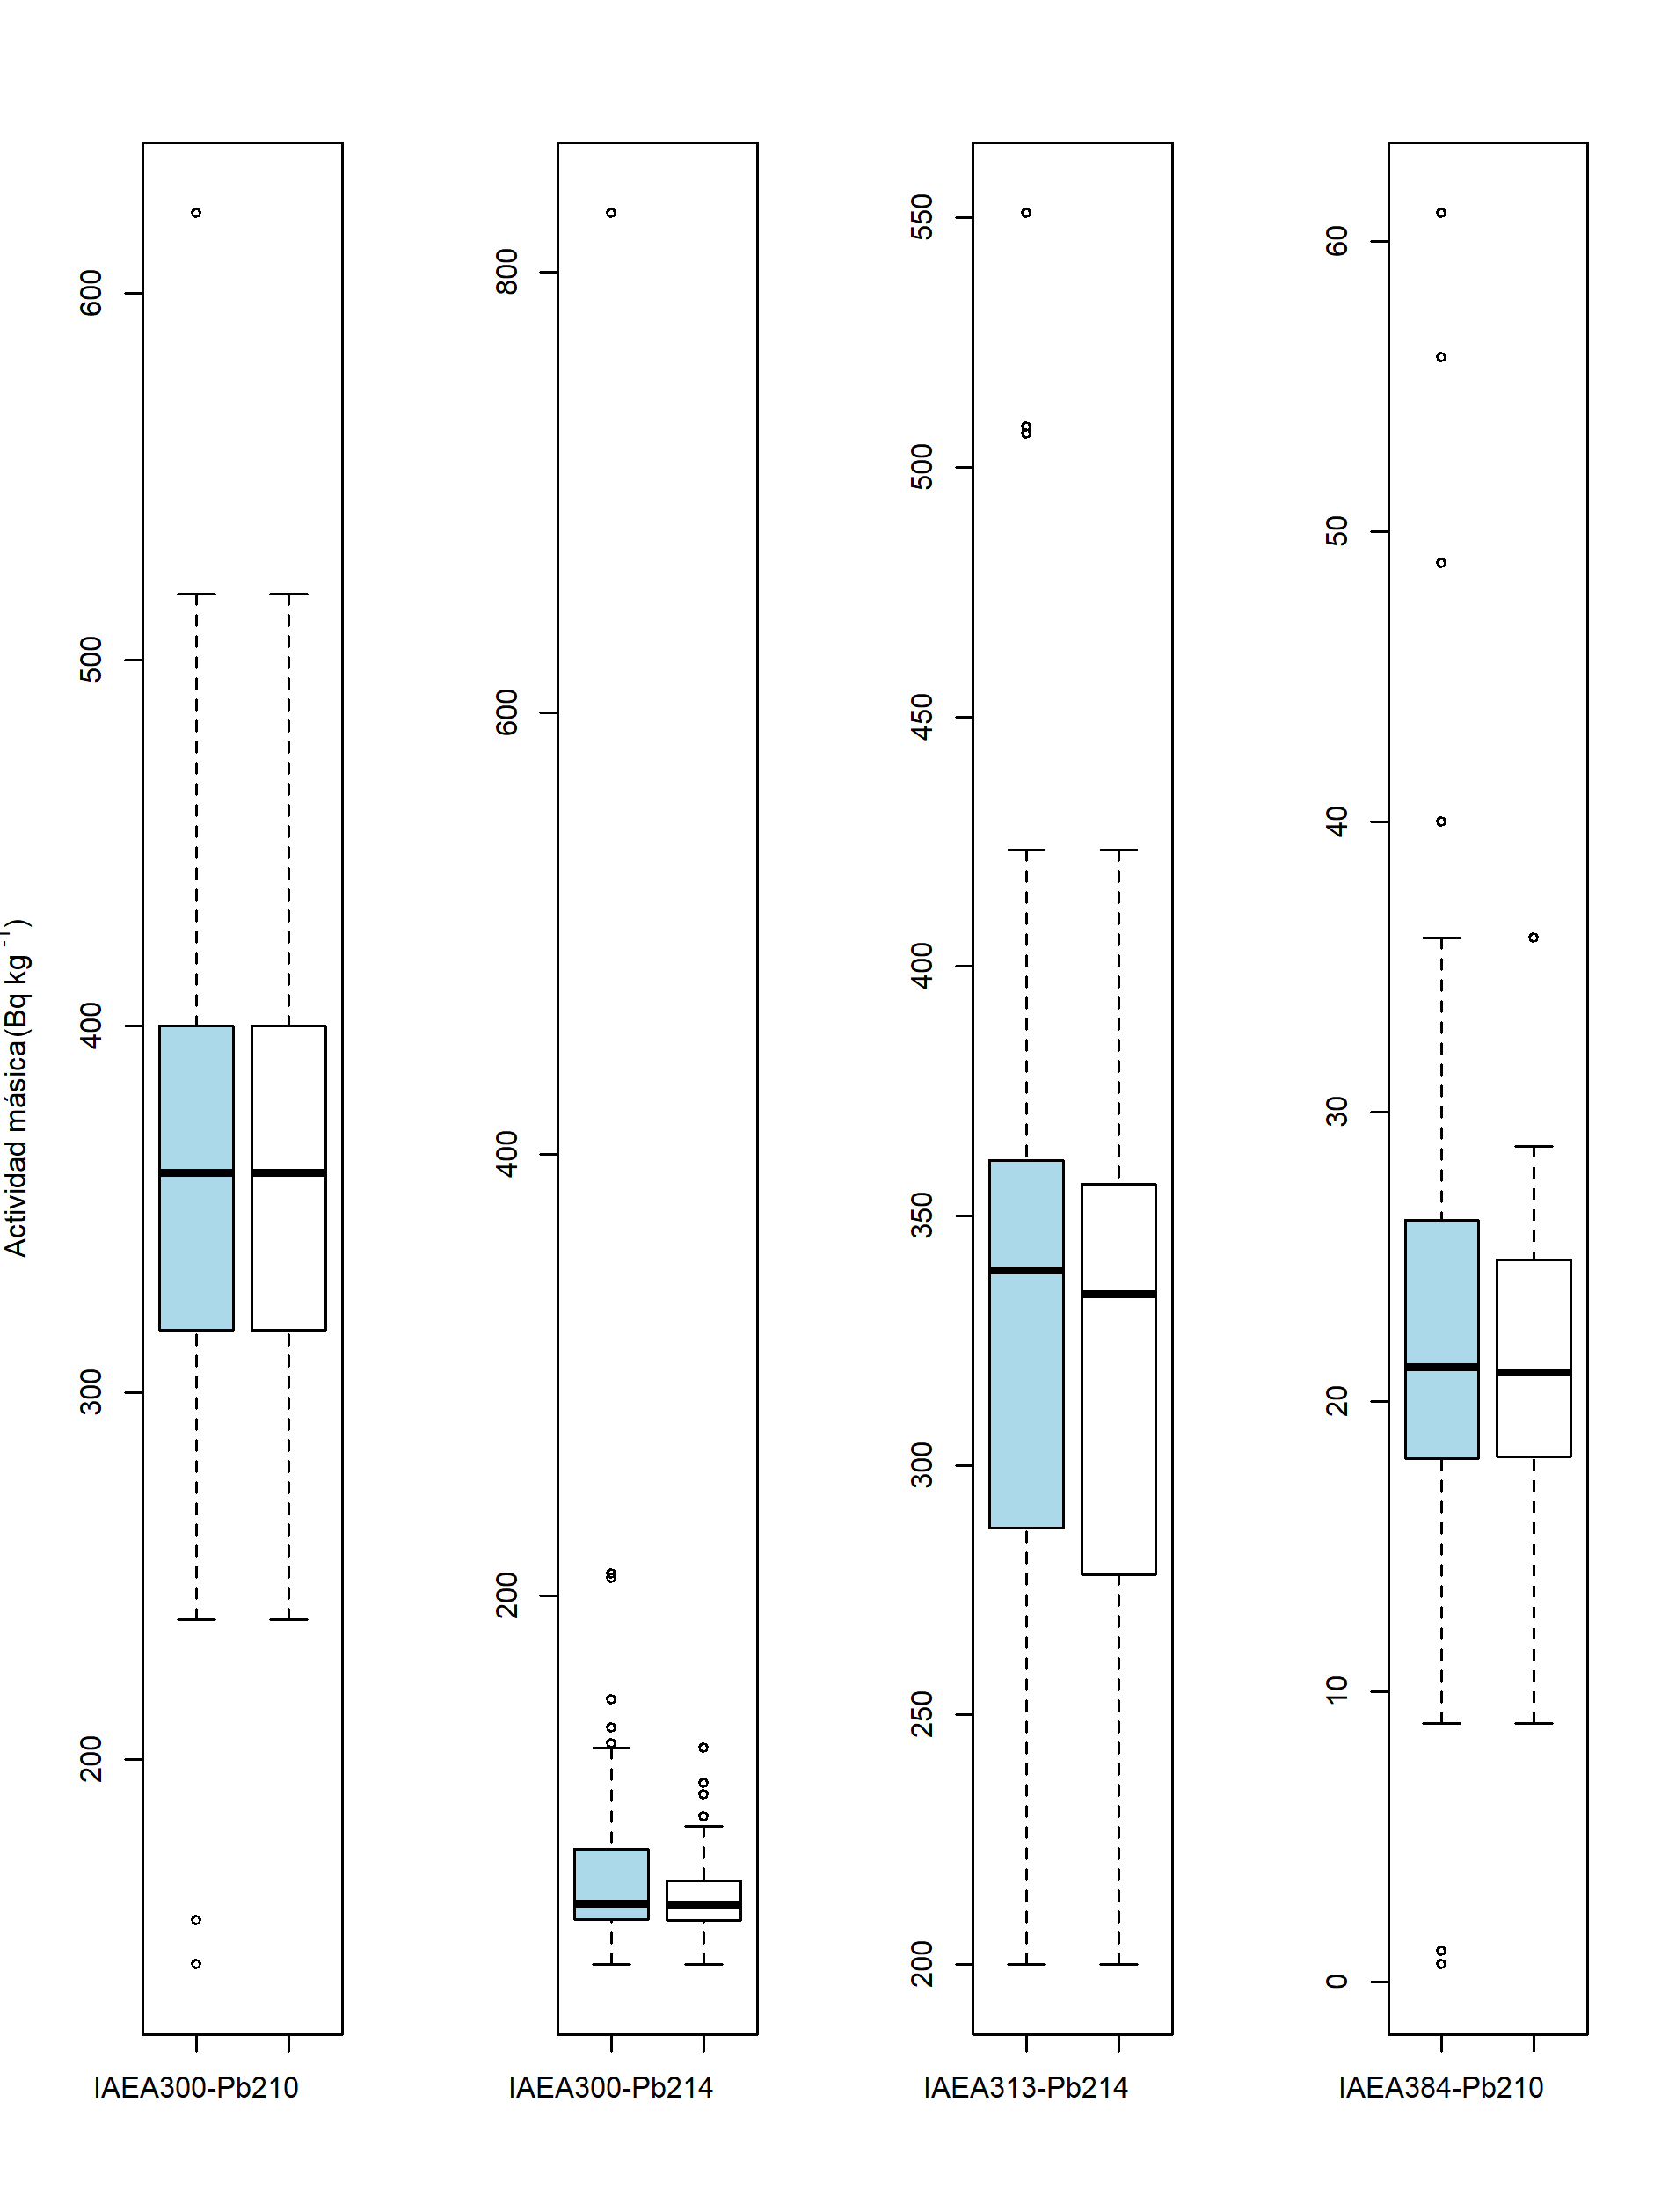
\includegraphics[width=0.9\textwidth]{Imagenes/PlotOutliers-1-IAEA-All.png}
\caption{Diagramas de cajas y valores atípicos de las actividades específicas de \PbCero\, y \PbCuatro\, reportadas para los materiales de referencias IAEA-300, IAEA-313 e IAEA-384. Izquierda: utilizando todos los valores reportados, derecha: excluyendo los primeros valores atípicos.  }\label{Fig-OutMRC-1}
\end{figure}
\begin{figure}
\centering 
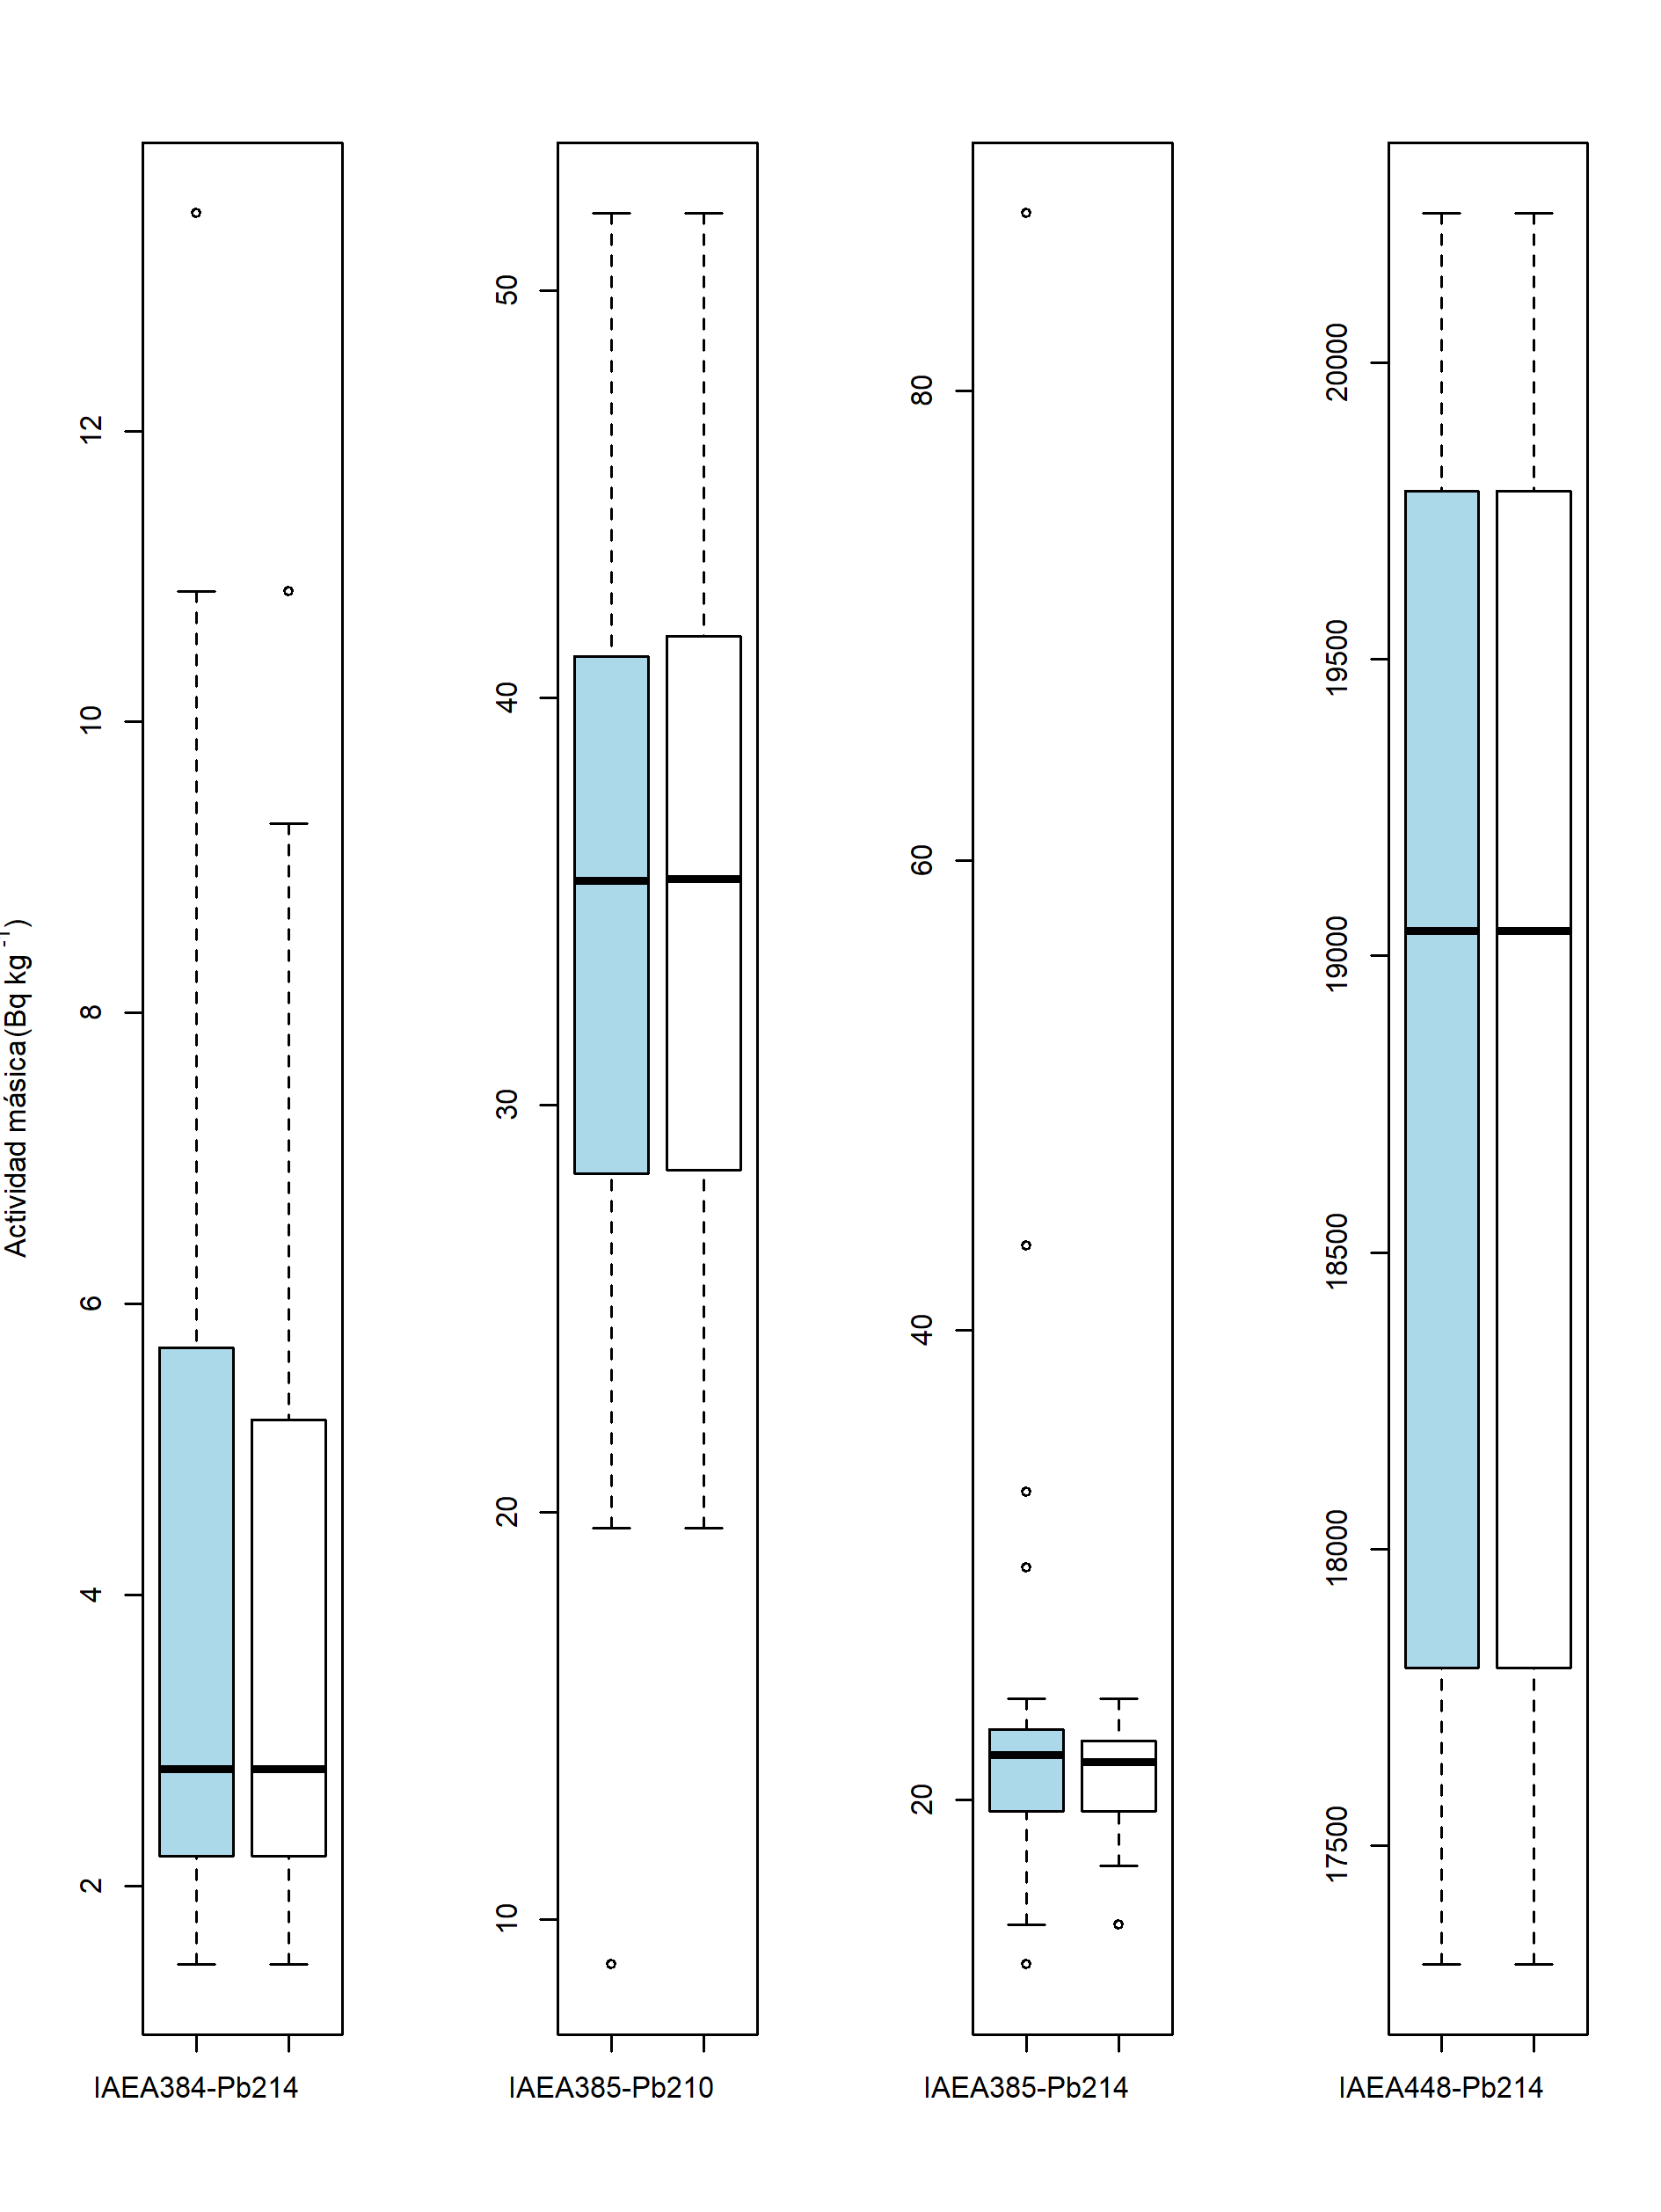
\includegraphics[width=0.9\textwidth]{Imagenes/PlotOutliers-2-IAEA-All.png}
\caption{Diagrama de cajas y valores atípicos de las actividades específicas de \PbCero\, y \PbCuatro\, reportadas para los materiales de referencias IAEA-384, IAEA-385 e IAEA-448. Izquierda: utilizando todos los valores reportados, derecha: excluyendo los primeros valores atípicos. }\label{Fig-OutMRC-2}
\end{figure}
\\
\\
Si se tiene $n$ mediciones de una variable tal que cada medición sea $x_i \pm \sigma_i$, $1\leq i\leq n$, entonces el promedio $\overline{x}$ y la desviación estándar total $\sigma$ es
\begin{eqnarray}
\overline{x} &=& \dfrac{1}{n}\sum_i^n x_i \\
\sigma^2_\text{int} &=& \dfrac{1}{n^2} \sum_i^n \sigma_i^2 \\
\sigma^2_\text{ext} &=& \dfrac{1}{n-1}\sum_i^n (x_i-\overline{x})^2 \\
\sigma &=& \sqrt{\sigma^2_\text{ext}  + \sigma^2_\text{int}}
\end{eqnarray}
donde $\sigma^2_\text{int}$ es la desviación estándar de todos los valores en relación a la media, y $\sigma^2_\text{ext}$ tiene en cuenta la incertidumbre de cada valor reportado. Los resultados se presentan en la Tabla \ref{Table-MRC}. 
\begin{table}
\centering
\caption{Actividad específica promedio $\overline{x}$ y desviación estándar $\sigma$ de Materiales de Referencia Certificados para \PbCero\, y \PbCuatro. Se incluye los valores de los percentiles 0.025 y 0.975}\label{Table-MRC}
\begin{tabular}{|c|c|c|c|c|c|}
\hline													
\rowcolor{Blue2}	MRC	&	No. de Datos	&	$\overline{x}$	&	$\sigma$	&	2.5 \% 	&	97.5 \% 	\\ 	\hline
\rowcolor{Blue1}	IAEA300-\PbCero	&	46	&	364.5	&	57.5	&	275.5	&	478.7	\\ 	
\rowcolor{Blue1}	IAEA300-\PbCuatro	&	66	&	65.1	&	19.7	&	38.8	&	111.9	\\ 	
\hline
\rowcolor{Blue1}	IAEA313-\PbCuatro	&	21	&	317.2	&	53.8	&	207.9	&	395.7	\\ 	
\hline
\rowcolor{Blue1}	IAEA384-\PbCero	&	29	&	21.2	&	5.6	&	11.1	&	31.0	\\ 	
\rowcolor{Blue1}	IAEA384-\PbCuatro	&	13	&	4.0	&	3.0	&	1.6	&	10.4	\\ 	
\hline
\rowcolor{Blue1}	IAEA385-\PbCero	&	44	&	35.1	&	7.8	&	22.4	&	46.0	\\ 	
\rowcolor{Blue1}	IAEA385-\PbCuatro	&	21	&	20.8	&	2.4	&	16.0	&	23.7	\\ 	
\hline
\rowcolor{Blue1}	IAEA448-\PbCuatro	&	6	&	18870.2	&	1202.3	&	17362.5	&	20194.3	\\ 	\hline
\end{tabular}
\end{table}
\section{Corrección y comparación de las actividades}
La Tabla \ref{Table-ZScoreResultados} muestra las actividades específicas de los MRC para la composición de referencia y la composición corregida. La composición corregida para los MRC se determinó de manera análoga al procedimiento descrito para las secciones de los núcleos sedimentarios (Sección \ref{Secc-100Composicion}) en donde se asume una composición estándar de 50 \% oxígeno. Estas actividades se encuentran corregidas para las fechas de referencia reportadas en los certificados de los materiales de referencia (Tabla \ref{Table-MRC}). 
\\
\\
La corrección en el tiempo de la actividad total de \PbCero\, ($^{210}$Pb$_\text{total}$) se realiza utilizando la ley de desintegración radiactiva y el semiperiodo $T_{\frac{1}{2}}$ adecuado para el \PbCeroBa\, y \PbCeroEx\, (Ecuación \ref{Eq-PbTotal}). Debido a la geoquímica de Pb, el semiperiodo de \PbCeroBa\, es el semiperiodo de \Ra\, (1600 años) \cite{DataDecayEvaluation} y el semiperiodo de \PbCeroEx\, corresponde al semiperiodo de \PbCero\, (22.23 años) \cite{DataDecayEvaluation}. 
\\
\\
Para la intercomparación de los resultados se utilizó $Z$-score, que se define como 
\begin{equation}\label{Eq-Zscore}
Z = \dfrac{| \overline{x} - \overline{x}_m | }{\sqrt{\sigma^2 + \sigma_m^2}}
\end{equation}
donde $\overline{x}$ y $\sigma$ es la actividad másica promedio y desviación estándar reportada (Tabla \ref{Table-MRC}), $\overline{x}_m$ y $\sigma_m$ es la actividad másica promedio y desviación estándar medida, asumiendo una composición de referencia o una composición corregida. Un resultado es aceptable si $Z \leq 2$, que equivale al criterio del 95 \%. \\
\begin{table}
\centering
\caption{Actividad y desviación estándar medida asumiendo una composición de referencia y la eficiencia de referencia y una referencia corregida por la composición. }\label{Table-ZScoreResultados}
\begin{tabular}{|c|c|c|c|cc|c|}
\hline																					
\rowcolor{Blue3}	MRC	&	Actividad certificado 			&	Actividad Ref.			&	Actividad Corr.			&	\multicolumn{2}{|c|}{$Z$}     			&	$\Delta Z$	\\	\hline
\rowcolor{Blue3}	IAEA-	&	Bq kg$^{-1}$			&	Bq kg$^{-1}$			&	Bq kg$^{-1}$			&	Ref.	&	Corr.	&		\\	\hline
\rowcolor{Blue2}	\multicolumn{7}{|l|}{\PbCero}     																			\\	\hline
\rowcolor{Blue1}	385	&	35.1 (7.8)			&	22.0 (11.3)			&	29.9 (13.4)			&	1.0	&	0.3	&	0.6	\\	
\rowcolor{Blue1}	384	&	21.2 (5.6)			&	26.7 (8.1)			&	36.1 (10.2)			&	0.6	&	1.3	&	-0.7	\\	
\rowcolor{Blue1}	300	&	364.5 (57.5)			&	183.8 (31.1)			&	227.5 (36.5)			&	2.8	&	2.0	&	0.8	\\	\hline
\rowcolor{Blue2}	\multicolumn{7}{|l|}{\PbCuatro}     																			\\	\hline
\rowcolor{Blue1}	313	&	317.2 (53.8)			&	327.1 (10.5)			&	337.4 (10.8)			&	0.2	&	0.4	&	-0.2	\\	\hline
\rowcolor{Blue1}	384	&	4.0 (3.0)			&	5.0 (0.7)			&	5.2 (0.7)			&	0.34	&	0.38	&	-0.04	\\	\hline
\rowcolor{Blue1}	300	&	65.1 (19.7)			&	49.9 (4.5)			&	50.6 (4.5)			&	0.7	&	0.7	&	0.0	\\	\hline
\rowcolor{Blue1}	385	&	20.8 (2.4)			&	25.0 (1.3)			&	25.7 (1.4)			&	1.5	&	1.8	&	-0.2	\\	\hline
\rowcolor{Blue1}	448	&	18870.2 (1202.3)			&	15732.7 (495.5)			&	16021.7 (504.6)			&	2.4	&	2.2	&	0.2	\\	\hline

\end{tabular}
\end{table}
\begin{figure}
\centering
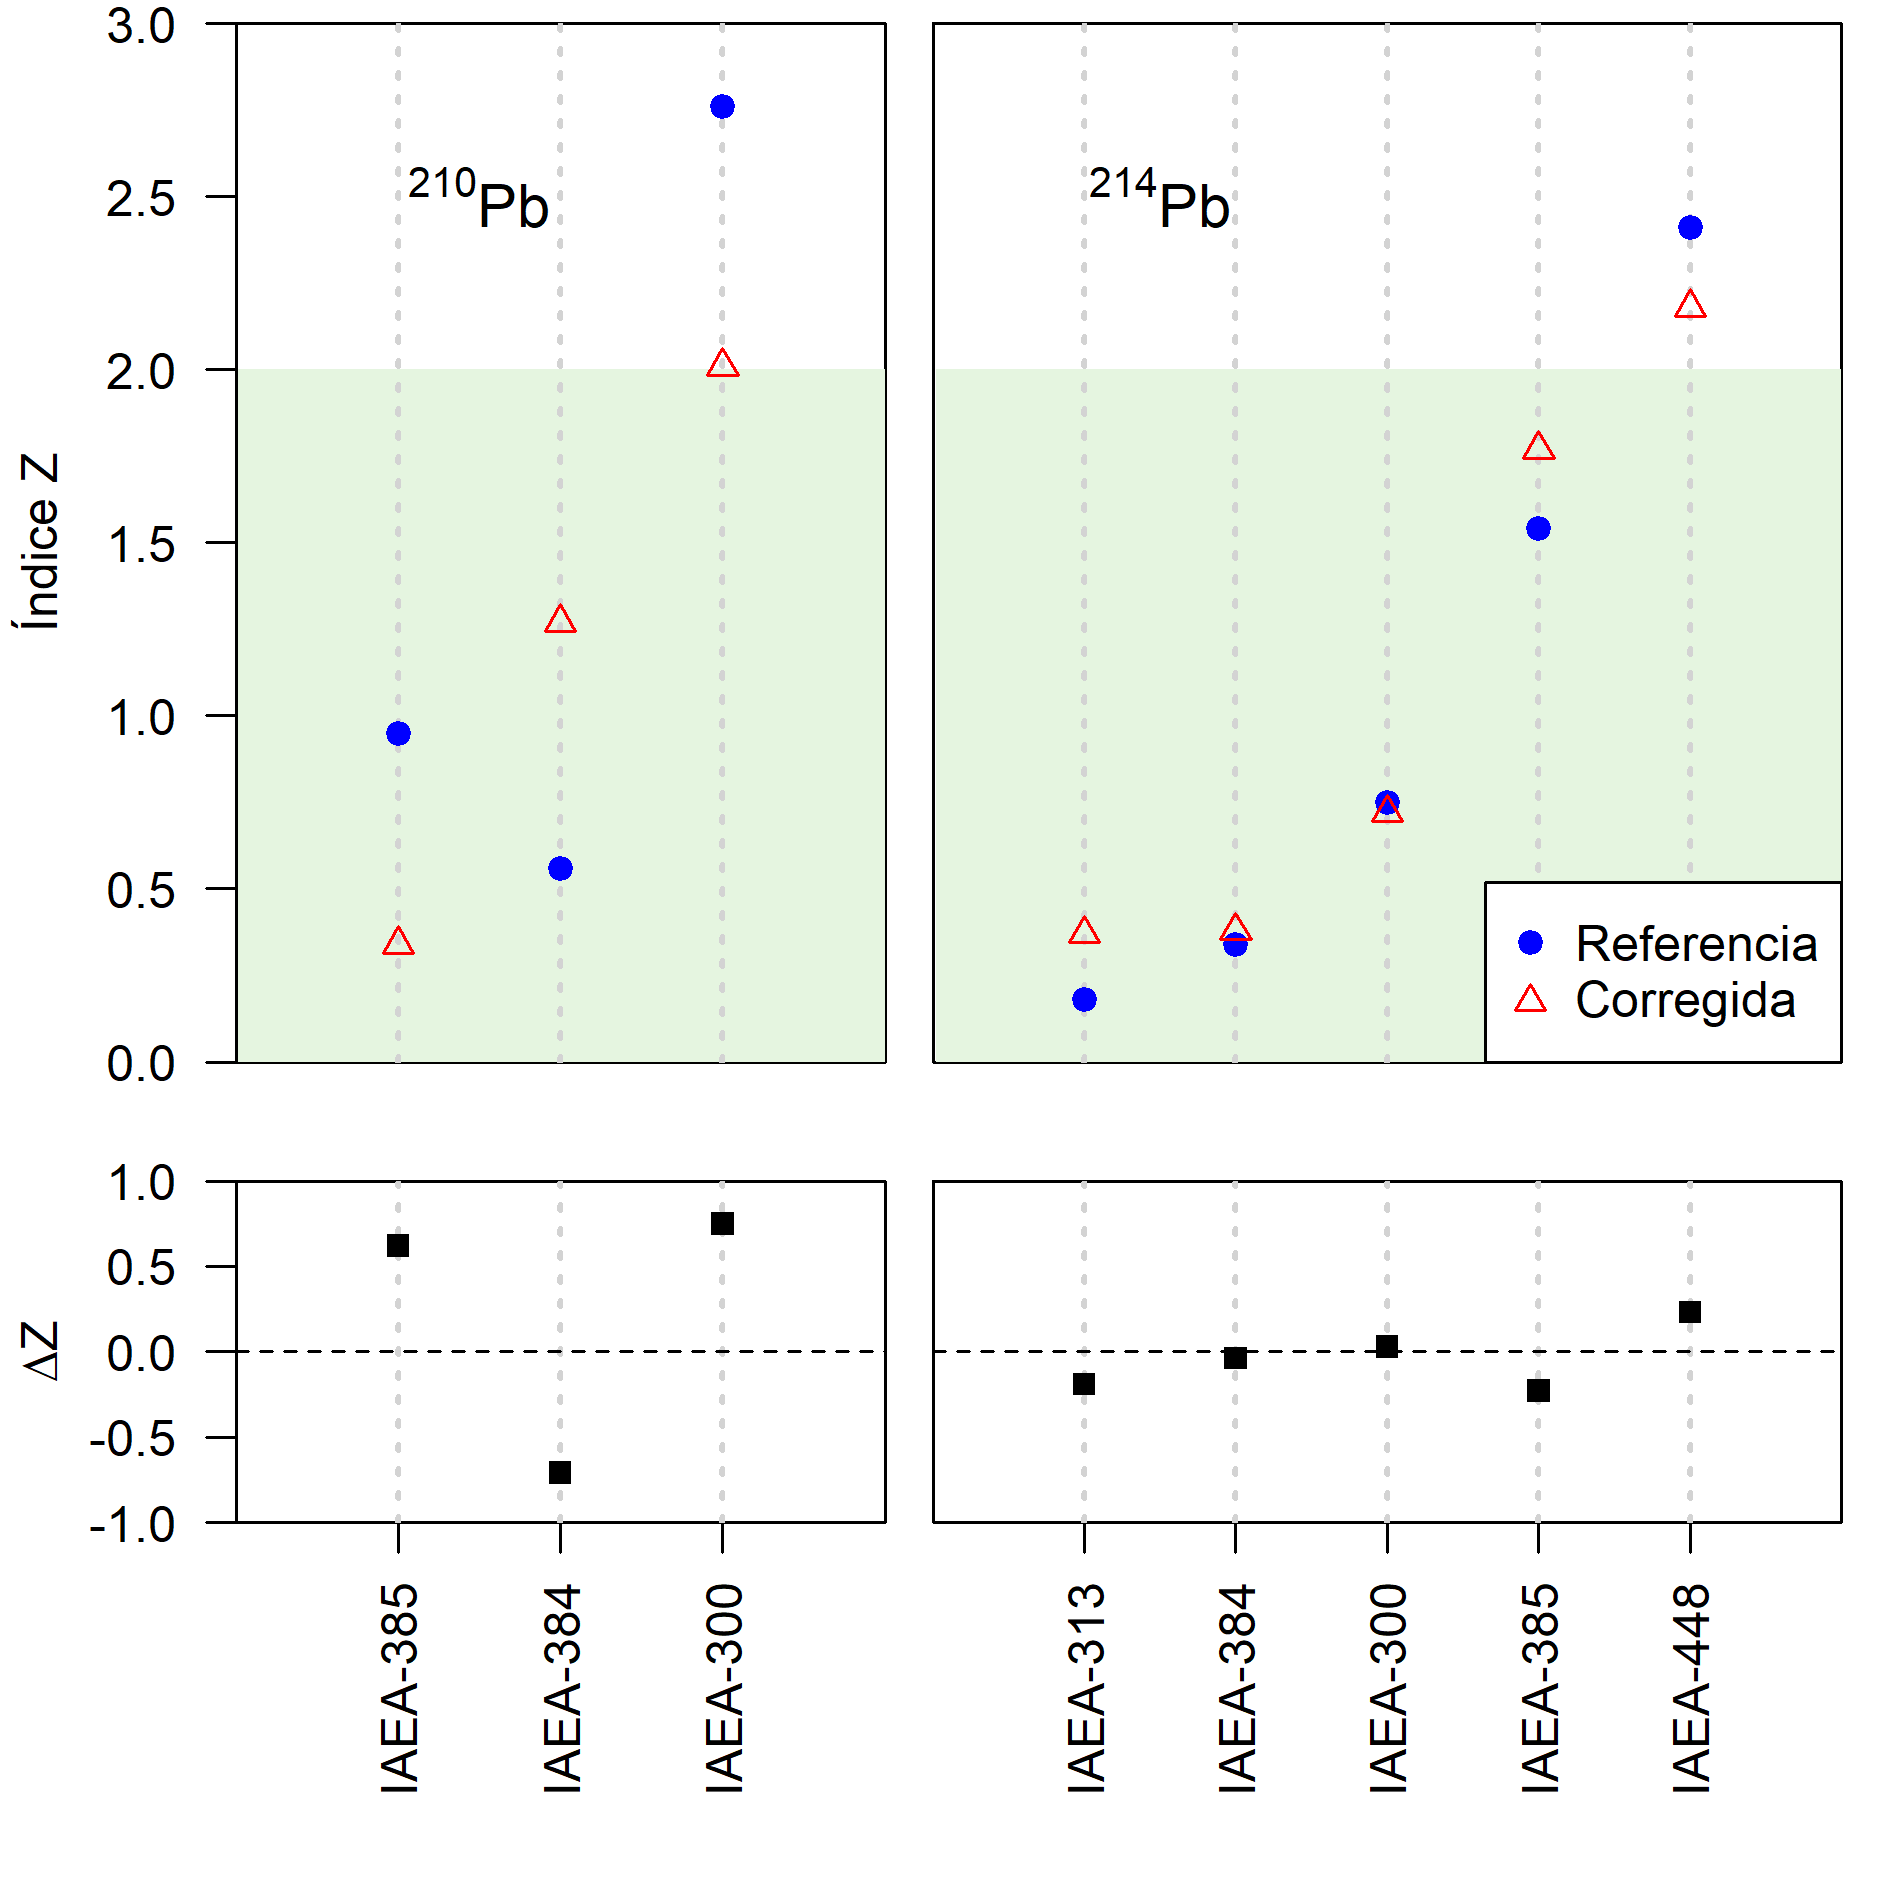
\includegraphics[width=0.9\textwidth]{Imagenes/Z-score-results.png}
\caption{Índice $Z$ y desviación $\Delta Z$ para las actividades másicas de materiales de referencia certificados utilizando una eficiencia de referencia y una eficiencia corregida por la composición.}\label{Fig-ZScore}
\end{figure}
\\De acuerdo a los resultados de la Tabla \ref{Table-ZScoreResultados} y a la Figura \ref{Fig-ZScore} se observa que dos (IAEA-385 e IAEA-384) de los tres MRC presentan resultados aceptables para \PbCero\, y cuatro (IAEA-313, IAEA-384, IAEA-300 E IAEA-385) de los cinco MRC presentan resultados aceptables para \PbCuatro\, puesto que el índice $Z$ es menor a dos en estos casos. 
\\ \\ 
También se observa que $\Delta Z$ para los resultados de las actividades utilizando una composición de referencia y una composición corregida es mayor para \PbCero\, ($|\Delta Z|$ > 0.5 en todos los casos) que para \PbCuatro\, ($|\Delta Z|$ < 0.5 en todos los casos). Lo anterior es debido a la dependencia de la eficiencia respecto a la composición - densidad para las energías relacionadas con los radionúclidos. 
\\ \\ 
La corrección de las actividades de \PbCero\, por la composición elemental disminuyó el índice $Z$ para los MRC IAEA-385 e IAEA-300 en comparación con los resultados en donde se utilizó una composición de referencia. Sin embargo, el MRC IAEA-384 produce mejores resultados cuando se asume una composición de referencia. Por otra parte, la corrección de las actividades de \PbCuatro\, por la composición elemental disminuye el índice $Z$ para los MRC IAEA-300 e IAEA-448. Para los MRC IAEA-313, IAEAE-384 e IAEA-385, los resultados producen menores índices Z cuando se asume una composición de referencia que cuando se asume una composición corregida, aunque ambas composiciones generan resultados aceptables ($Z$ < 2). 
\\ \\ 
En los resultados del índice $Z$ para los dos radionúclidos (\PbCero\, y \PbCuatro) se observa que IAEA-384 e IAEA-300 presentan el mismo comportamiento aunque diferentes $\Delta Z$. El índice $Z$ es mayor tanto para la actividad corregida de \PbCero\, y \PbCuatro\, en IAEA-384, como para la actividad de referencia en IAEA-300. En contraste, para el MRC IAEA-385, los índices $Z$ fueron menores para las actividades de \PbCero\, corregidas por la composición elemental, así como para las actividades \PbCuatro\, determinadas a partir de una composición de referencia.